\documentclass[../main.tex]{subfiles}
\graphicspath{{\subfix{../figures/}}}

\begin{document}
    Im Folgenden wird ein erweitertes Modell erstellt, das auf dem SIR-Modell aus Abschnitt \ref{sec:basic_model} basiert und dieses um drei wichtige Aspekte ergänzt.

    \subsection{Anpassung der Annahmen}
    \label{ssec:assumptions2}
    \paragraph{Impfungen werden durchgeführt.} 
    Diese verleihen Immunität, was dem Übergang $S \to R$ entspricht. Es wird täglich ein konstanter Anteil $\zeta = 1.4 \cdot 10^{-3}$ der Bevölkerung geimpft. Damit $s$ nicht negativ werden kann, beschreiben wir den Übergang  mit der Funktion $\eta(s)$:
    \begin{equation}
        \eta(s) = 
        \begin{cases}
            \zeta, &\text{wenn } s \geq \zeta \\
            s      &\text{andernfalls}
        \end{cases}
    \end{equation}

    \paragraph{Immunität ist temporär.} 
    Sie verschwindet nach 90 Tagen, was dem Übergang $R \to S$ entspricht. Hierbei handelt es sich um einen Übergang nach konstanter Aufenthaltsdauer, der daher mit dem mathematischen Ausdruck $\alpha r$ für $\alpha = \frac{1}{90}$ beschrieben wird.

    \paragraph{Saisonalität beeinflusst die Ausbreitung.} 
    Die Kontagiosität von Covid-19 weist jahreszeitliche Schwankungen um den Faktor $\xi = 0.46$ auf. Auf der Nordhalbkugel ist sie im Winter um $\beta \xi$ erhöht und im Sommer um $\beta \xi$ gesenkt. Dies betrifft den Übergang $S \to I$ mit dem bisherigen Ausdruck der Inzidenz $\beta s i$. Im Folgenden ersetzen wir $\beta$ durch eine zeitabhängige Funktion $\lambda(t)$ mit einer Periode von 365 und der Wertemenge $\mathbb{W}_\lambda = [\beta - \beta \xi;\ \beta + \beta \xi] =  [\beta(1-\xi);\ \beta(1+\xi)]$:
    \begin{equation}
        \lambda(t) = \beta \cdot \left(1 + \xi \cdot \sin \left(\frac{2\pi t}{365}\right) \right)
    \end{equation}

    Auch das erweiterte Modell kann in einem Transferdiagramm (Abbildung \ref{fig:extended_sir_transfer}) dargestellt werden. Da eine Infektion keine dauerhafte Immunität verleiht und Individuen wieder aus $R$ nach $S$ wechseln, spricht man von einem SIRS-Modell.

    \begin{figure}[h]
        \centering
        \begin{tikzpicture}
            \tikzmath{\bl=1.5; \al=4;}

            \foreach \t\n in {S/0, I/1, R/2}
                \tikzmath{
                    \x = \n*\bl + \n*\al;
                    \y = -0.5*\bl;
                }
                \draw (\x, \y) rectangle node{\t} (\x+\bl, \y+\bl);

            \foreach \t\n in {Infektion ($\lambda_{(t)} s i$)/0, Genesung ($\gamma i$)/1}
                \tikzmath{\x = \bl + \n*\bl + \n*\al;}
                \draw[-{>[scale=2]}] (\x, 0) -- node[auto]{\t} (\x+\al, 0);

            \draw[-{>[scale=2]}] (0.5*\bl, 0.5*\bl) -- (0.5*\bl, 1.5*\bl) -- node[auto]{Impfungen ($\eta_{(s)}$)} (2.5*\bl+2*\al, 1.5*\bl) -- (2.5*\bl+2*\al, 0.5*\bl);

            \draw[-{>[scale=2]}] (2.5*\bl+2*\al, -0.5*\bl) -- (2.5*\bl+2*\al, -1.5*\bl) -- node[auto]{Immunitätsverlust ($\alpha r$)} (0.5*\bl, -1.5*\bl) -- (0.5*\bl, -0.5*\bl);
        \end{tikzpicture}
        \caption{Transferdiagramm: Erweitertes Modell}
        \label{fig:extended_sir_transfer}
    \end{figure}

    
    \subsection{Definition des Modells}
    \label{ssec:definition2}

    Bei dem erweiterten Modell handelt es sich um ein SIRS-Modell mit Impfungen und Saisonalität. 
    
    Es wird durch folgendes Differentialgleichungssystem definiert:
    \begin{equation}
        \label{eq:sir_extended}
        \setlength{\jot}{0.5cm}
        \begin{aligned}
            \frac{ds}{dt} &= - \lambda_{(t)} s i - \eta_{(s)} + \alpha r, \\
            \frac{di}{dt} &= \lambda_{(t)} s i - \gamma i, \\
            \frac{dr}{dt} &= \gamma i + \eta_{(s)} - \alpha r \\
            &\text{mit } \lambda_{(t)} = \beta \cdot \left(1 + \xi \cdot \sin \left(\frac{2\pi t}{365}\right) \right) \\
            &\text{und } \eta_{(s)} = 
                \begin{cases}
                    \zeta, &\text{wenn } s \geq \zeta \\
                    s      &\text{andernfalls}
                \end{cases}
        \end{aligned}
    \end{equation}

    Es gelten die Anfangsbedingungen aus Tabelle \ref{tab:initial_state}:
    \begin{equation*}
        \begin{aligned}
        &s_0 = 3.13 \cdot 10^{-1}, \\
        &i_0 = 1.36 \cdot 10^{-2}, \\
        &r_0 = 6.73 \cdot 10^{-1}
        \end{aligned}
    \end{equation*}

    Betrachten wir $\lambda(t)$ für $t=0$, so ergibt sich $\lambda(0) = \beta$  sowie  $\lambda'(0)>0$. Dies ist genau zum Anfangszeitpunkt, dem 30. September, der Fall, sodass die Simulation mit $t=0$ startet.
    
    Eine Übersicht über die Parameter mit den in Abschnitt \ref{ssec:epidemiological_aspects} gewählten Werten findet sich in Tabelle \ref{tab:parameters}.

    Durch Berücksichtigung der Saisonalität tritt die Zeit im Diffenzialgleichungssystem \eqref{eq:sir_extended} des erweiterten Modells explizit auf, sodass dieses nicht mehr autonom ist. Je nach Anfangszeitpunkt entwickelt sich sein Zustand daher unterschiedlich.

    \begin{table}[h]
        \centering
        \begin{tabularx}{\textwidth}{X | p{.5\textwidth} | X}
            \textbf{Symbol}     & \textbf{Erklärung}    & \textbf{Wert}         \\ \hline
            $\beta$             & Infektionsrate        & $0.95$                \\ \hline
            $\frac{1}{\gamma}$  & Infektionsdauer       & $10$                  \\
            $\gamma$            & Genesungsrate         & $\frac{1}{10}$        \\ \hline
            $\frac{1}{\alpha}$  & Immunitätsdauer       & $90$                  \\
            $\alpha$            & Immunitätsverlustrate & $\frac{1}{90}$        \\ \hline
            $\zeta$             & Impfrate              & $1.4 \cdot 10^{-3}$   \\ \hline
            $\xi$               & Saisonalitätsfaktor   & $0.46$
        \end{tabularx}
        \caption{Übersicht über Parameter}
        \label{tab:parameters}
    \end{table}

    \subsection{Simulation von Szenarien}
    \label{ssec:simulation2}
    Im Folgenden werden mehrere Szenarien des erweiterten Modells \eqref{eq:sir_extended} simuliert\footnote{Informationen zur verwendeten Software im Anhang (S. \pageref{ap:simulation})}.
    Für die Parameter gelten die Werte aus Tabelle \ref{tab:parameters}, welche, wie im Verlauf beschrieben, variiert werden.

    Die Simulation wird anhand der Zeitreihe der Gruppengrößen visualisiert. Darunter befindet sich mit identischer Zeitachse die Zeitreihe der effektiven Reproduktionszahl, wodurch die Entwicklung des Systems besser nachvollziehbar ist. Rechts davon wird der Verlauf in der SI-Phasenebene dargestellt, wobei die horizontale Achse den Anteil der Suszeptiblen und die vertikale Achse den Anteil der Infizierten zeigt.

    \paragraph{Szenario 1: Standard}
    Hierbei handelt es sich um den erwarteten Verlauf (Abbildung \ref{fig:sim_default}). Wir betrachten für $\xi=0$ zudem das fiktive Szenario ohne Saisonalität, bei dem es sich wieder um ein autonomes System handelt (Abbildung \ref{fig:sim_no_seasonality}).
    \begin{figure}
        \centerline{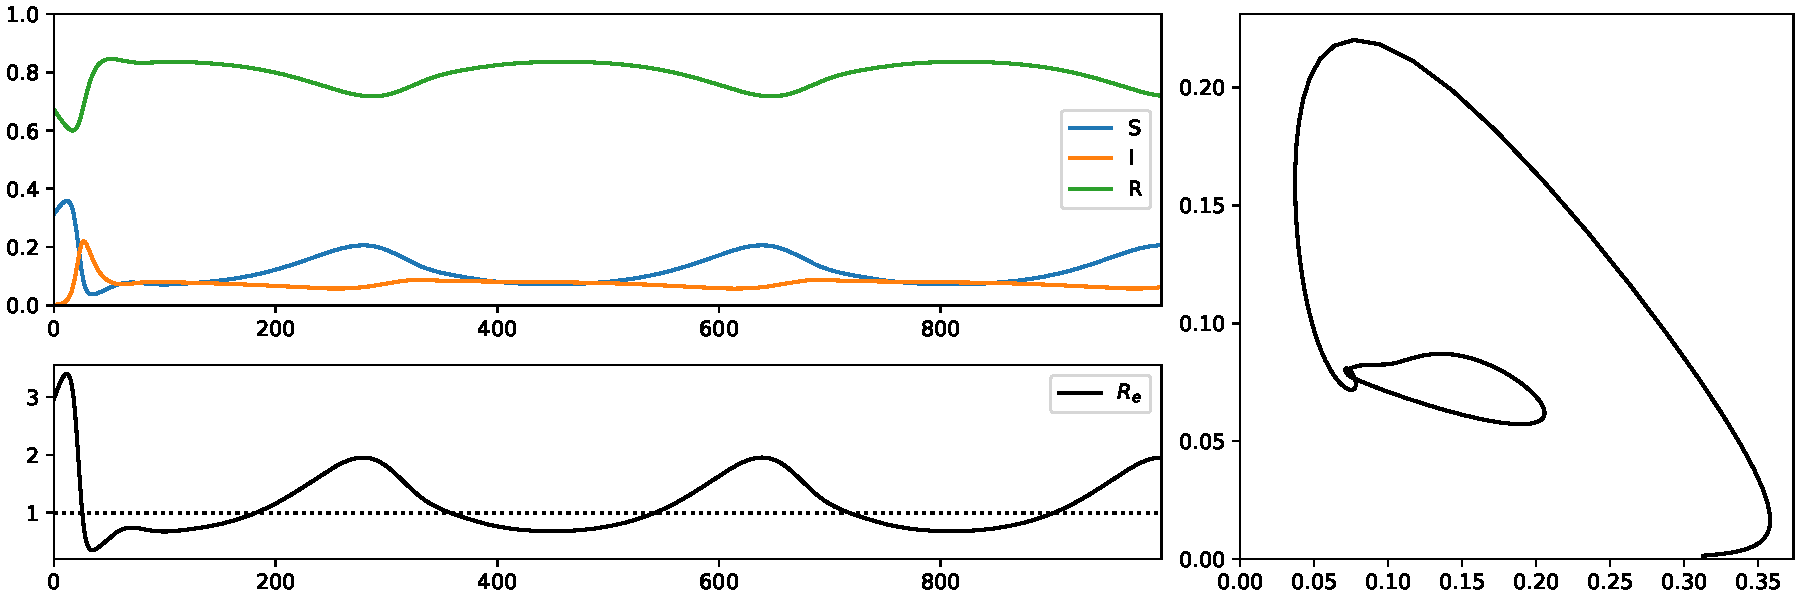
\includegraphics[width=1.4\textwidth]{simulations/default.pdf}}
        \caption[Verlauf des erweiterten Modells: Standard]{Verlauf des erweiterten Modells: Standard \\ $i_{max}=0.22$; $I_{max}=1.83 \cdot 10^7$ für $t=27$}
        \label{fig:sim_default}
    \end{figure}
    \begin{figure}
        \centerline{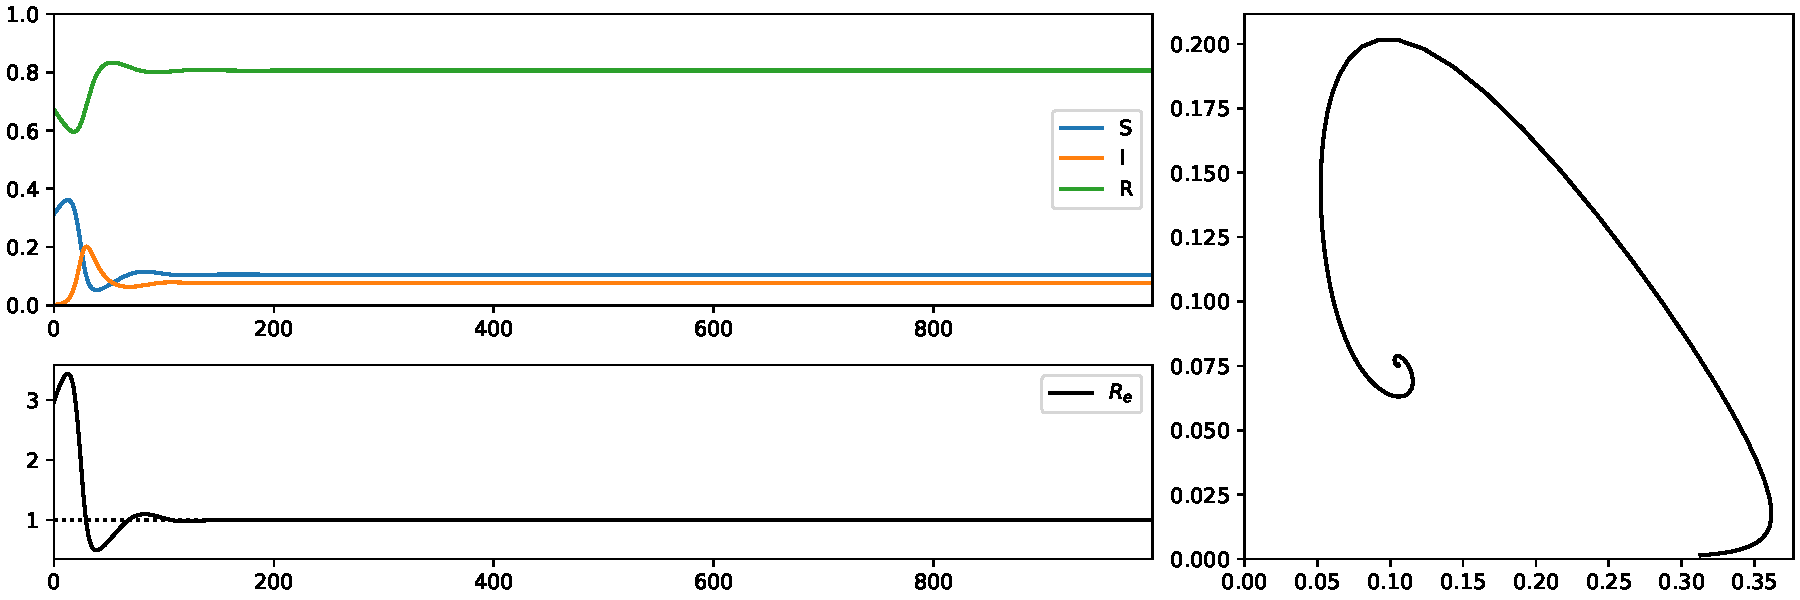
\includegraphics[width=1.4\textwidth]{simulations/no_seasonality.pdf}}
        \caption[Verlauf des erweiterten Modells: Ohne Saisonalität]{Verlauf des erweiterten Modells: Ohne Saisonalität \\ $i_{max}=0.2$; $I_{max}=1.67 \cdot 10^7$ für $t=30$}
        \label{fig:sim_no_seasonality}
    \end{figure}
     
    \paragraph{Szenario 2: Erhöhte Impfrate}
    In diesem Szenario erhöht sich die Impfrate auf $\zeta=0.0042$ (Abbildung \ref{fig:sim_vaccinations_up}).
    \begin{figure}
        \centerline{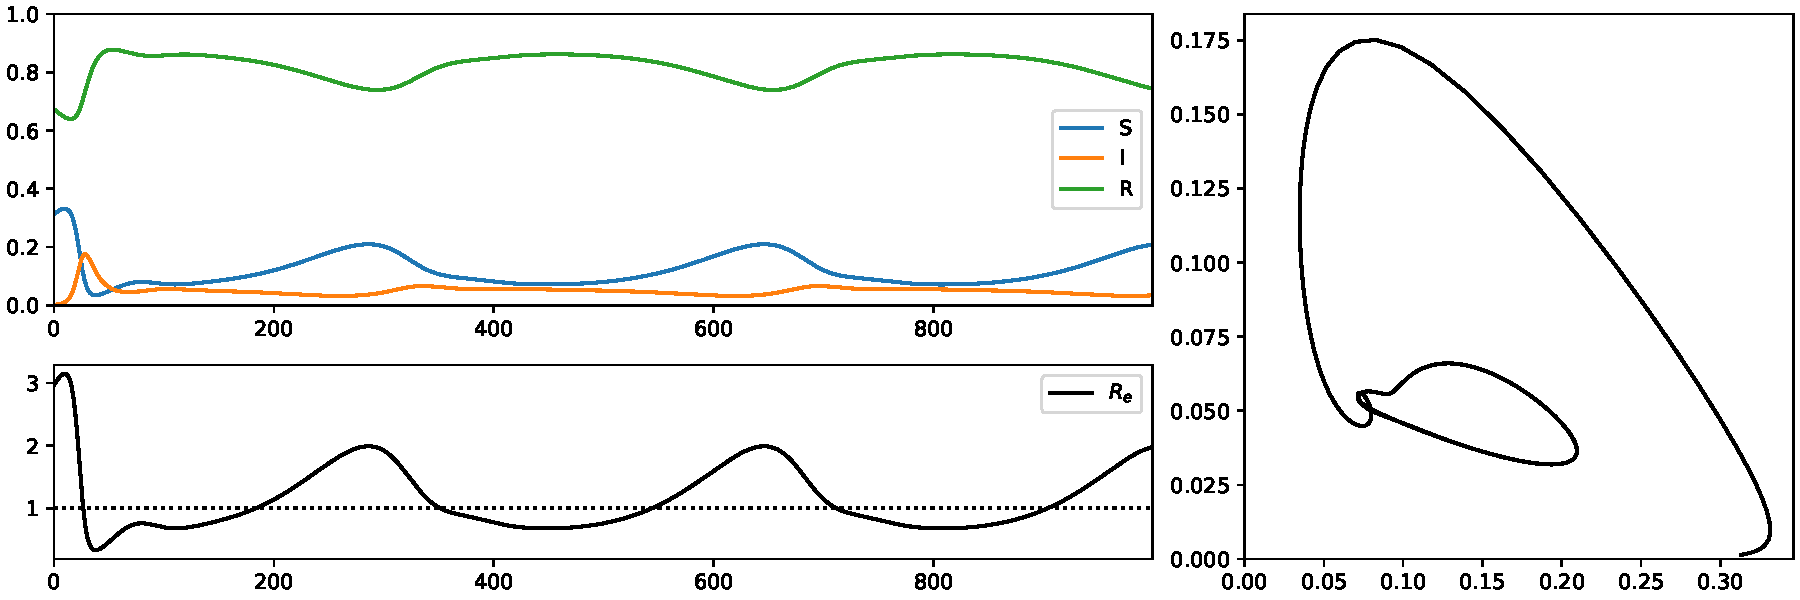
\includegraphics[width=1.4\textwidth]{simulations/vaccinations_up.pdf}}
        \caption[Verlauf des erweiterten Modells: Erhöhte Impfrate]{Verlauf des erweiterten Modells: Erhöhte Impfrate \\ $i_{max}=0.18$; $I_{max}=1.45 \cdot 10^7$ für $t=28$}
        \label{fig:sim_vaccinations_up}
    \end{figure}

    \paragraph{Szenario 3: Gesenkte Infektionsrate}
    In diesem Szenario sinkt die Infektionsrate auf $\beta=0.4$ (Abbildung \ref{fig:sim_infectiosity_down}). Dies kann durch Eindämmungsmaßnahmen wie Kontaktreduzierung und das Tragen von Masken geschehen.
    \begin{figure}
        \centerline{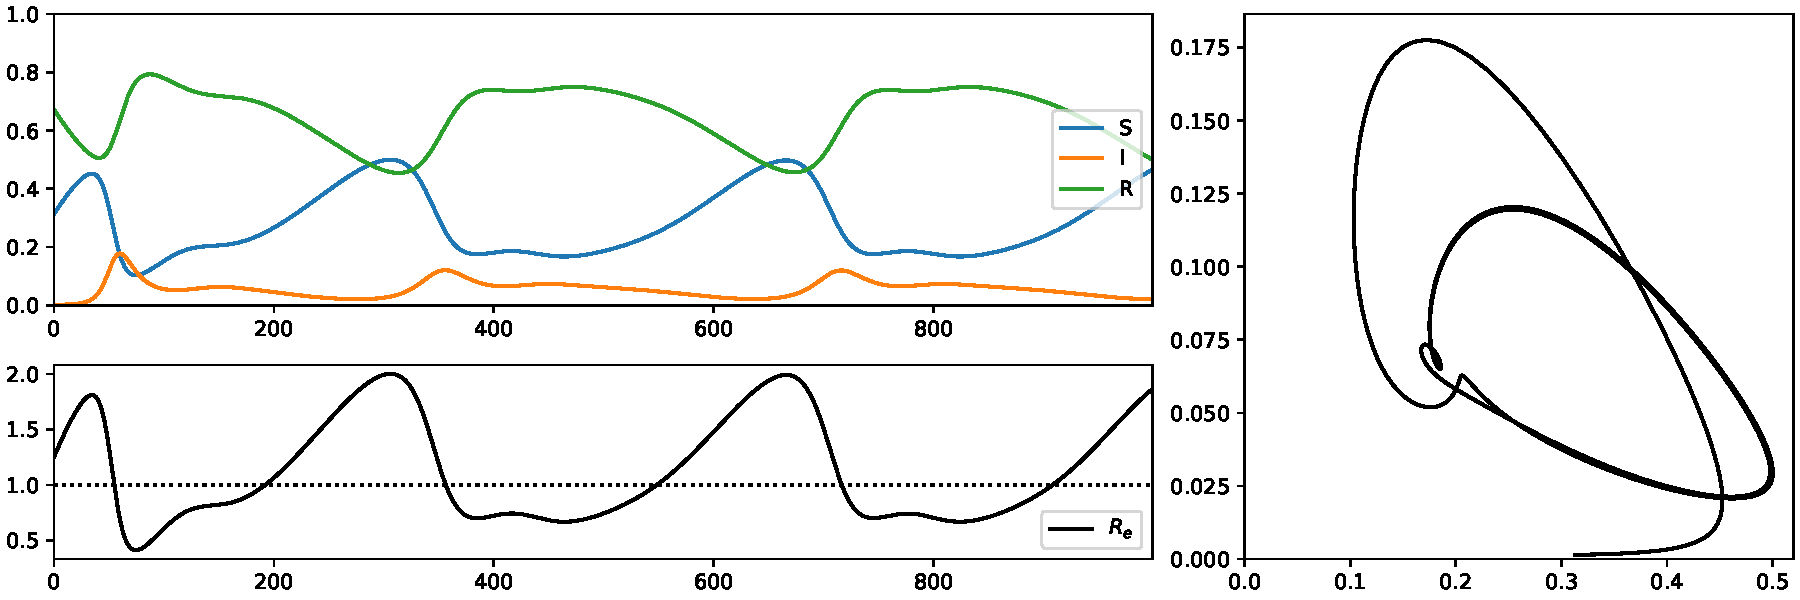
\includegraphics[width=1.4\textwidth]{simulations/infectiosity_down.pdf}}
        \caption[Verlauf des erweiterten Modells: Gesenkte Infektionsrate]{Verlauf des erweiterten Modells: Gesenkte Infektionsrate \\ $i_{max}=0.18$; $I_{max}=1.47 \cdot 10^7$ für $t=60$}
        \label{fig:sim_infectiosity_down}
    \end{figure}


    \subsection{Auswertung der Simulation}
    Im folgenden werden aus den simulierten Szenarien Rückschlüsse auf die Realität gezogen.

    Im Standardszenario kommt es zeitnah zu einer Welle, die mit über 18 Millionen Infizierten das größte Ausmaß während der simulierten Zeitspanne besitzt. Dieser Wert, der bei einer ungebremsten Ausbreitung eintritt, würde das Gesundheitssystem überlasten, wofür die Grenze von 15 Millionen Infizierten bestimmt wurde.
    In den folgenden Jahren treten im Winter periodisch Wellen auf, die etwa 10\% der Bevölkerung infizieren, damit nicht zu einer Überlastung führen und ein gleichbleibendes Ausmaß aufweisen. Diese Wellen zeigen sich in der Phasenebene in der länglichen Schleife, welche die Trajektorie wiederholt durchläuft. Die Entwicklung lässt sich insbesondere im Verlauf der effektiven Reproduktionszahl $R_e$ nachvollziehen, die den kritischen Wert von eins überschreitet, sobald sich eine neue Welle anbahnt und anschließend wieder unter eins fällt. Eine Endemie bezeichnet eine Krankheit, die heimisch geworden ist und zeitlich unbegrenzt auftritt. Dabei besteht in der Population bereits Immunität, sodass die Krankheit leichtere Verläufe hervorruft und das Ausmaß ihrer Wellen unter dem einer Epidemie liegt. Da die Krankheit in der Simulation dauerhaft unter dem Niveau der ersten Welle bestehen bleibt, ist von einer Endemisierung von Covid-19 ausgehen.

    Im fiktiven Szenario ohne Saisonalität stellt sich nach der ersten Welle ein Gleichgewichtszustand ein, der sich durch das Einpendeln von $R_e$ bei eins sowie in der Phasenebene durch die spiralförmige Annäherung an den Gleichgewichtszustand zeigt.

    Die bei Saisonalität auftretenden periodischen Wellen lassen sich damit wie folgt erklären: Die im Sommer gesenkte Kontagiosität führt zu einem Rückgang der Infektionszahlen und verzögert auch zum Absinken des Immunitätsanteils. Dadurch kommt es im Winter bei erhöhter Kontagiosität erneut zu einer Welle.

    Die Szenarien mit erhöhter Impfrate beziehungsweise gesenkter Infektionsrate zeigen, dass der Anteil der Infizierten am Höhepunkt der ersten Welle durch beide Maßnahmen so gesenkt werden kann, dass keine Überlastungssituation mehr eintritt. Eine Verzögerung des Höhepunkts der ersten Welle kann aber nur durch eine Senkung der Infektionsrate, das heißt durch Eindämmungsmaßnahmen, erreicht werden. Der Höhepunkt wurde dann erst an Tag 60 statt an Tag 27 wie im Standardszenario erreicht. Der entscheidende Unterschied zeigt sich auf lange Sicht in den periodisch auftretenden Wellen. Deren Ausmaß wird nur durch eine erhöhte Impfrate verringert, wie in der Phasenebene an der nach unten verschobenen Schleife mit geringerem Ausmaß in vertikaler i-Richtung zu erkennen ist. Eine Senkung der Infektionsrate, die zudem mit gesellschaftlichem Schaden einhergeht, zeigt hier keine Wirkung.
    Dies unterstreicht die Bedeutung von Impfungen für die Kontrolle von Covid-19.
\end{document}